
\subsubsection{FFT}
\\
The energy, delay and area estimates for each architecture / frequency combination is given in TABLE VI.
In Fig. 8, Fig. 9 we show the Power-Delay and Area-Delay plot for FFT.

\begin{table}[ht]
\caption{Energy / Delay / Area for each architecture/frequency combination}
\begin{center}
\begin{tabular}{c | c   c   c   c    c   c}
\hline
FFT &1x2 &1x0 &2x0 &2x2 &4x2 &4x0 \\ [1ex]
\hline
Frequency (MHz) &41.66 &41.67& 41.66& 45.45& 45.45&45.45 \\ [1ex] 
Energy (uJ)&24.65 &14.71 &31.04 &16.7 &41.38 &18.55 \\ [1ex]

Delay (us)& 203.792& 154.88& 189.27& 141.606& 172.453& 140.55\\[1ex] 
Area (mm^2)& 5.4& 5.07 & 6.6& 5.7& 9.2& 6.7\\[1ex]
\hline

\end{tabular}}
\label{diffstruc}
\end{center}
\end{table}


\begin{figure}[ht]
{\centering \resizebox*{6in}{4in}{\includegraphics{fftp.ps}} \par}
\caption{Power-Delay plot for FFT}
\end{figure}

\begin{figure}[ht]
{\centering \resizebox*{6in}{4in}{\includegraphics{ffta.ps}} \par}
\caption{Area-Delay plot for FFT}
\end{figure}


